% Provenance (never printed): see sources/outline_sources.md (Year 3:
% stereographic projection; fold and fault analysis; palaeostress; balanced
% cross-sections). Brief: sources/book5/BRIEFS.md, ch. 8. Nets, pi-diagram and
% fault-slip data from figdata/bachelor-3/stereonet.py (Varden data invented,
% from figdata/shared/region.py); Fry plot from figdata/bachelor-3/fry.py.
% Exercise and problem values in the Book 5 scratch calculator calc/ch08.py.
% No real-world numbers: no ledger rows.
\chapter{Análise estrutural}\label{ch:b3:structural-analysis}

Um geólogo mediu duzentos planos de acamamento nos flancos de uma dobra
grande demais para ser vista por inteiro: sua charneira está sob uma floresta, e seus flancos se estendem por
quilômetros. Cada leitura é um par de números. Representadas como pontos em uma carta circular,
os \omterm{def:b3:structural-analysis:stereo}{polos} dos planos caem ao longo de uma única curva, um círculo máximo, e
o \omterm{def:b3:structural-analysis:stereo}{polo} desse círculo máximo é o eixo da dobra, uma reta que ninguém
jamais viu. Este capítulo constrói a carta, a \omterm{def:b3:structural-analysis:stereo}{projeção estereográfica}, e
usa-a, com as ferramentas vetoriais que a sustentam, para encontrar eixos de dobras, para medir a
deformação registrada por objetos deformados, para recuperar a tensão que impulsionou um conjunto de
falhas, e para restaurar uma seção geológica deformada ao seu estado anterior à
deformação.

\begin{recall}
Os círculos máximos e menores de uma esfera estão no volume do primeiro ano, no capítulo
sobre astronomia esférica; direção, mergulho, sentido de mergulho, rumo e caimento, nos seus capítulos
sobre mapas geológicos e seções geológicas; a normal unitária ascendente de um
plano de sentido de mergulho $\alpha$ e mergulho $\delta$, $\vec n = (\sin\delta
\sin\alpha, \sin\delta\cos\alpha, \cos\delta)$ nas direções leste, norte e para cima
as componentes, e a média vetorial de um conjunto de medidas no seu primeiro capítulo sobre
métodos de campo e de laboratório. Elementos e classes de dobras, a linha de charneira de uma
dobra paralela a $\vec n_1\times\vec n_2$ e o ângulo interflancos
$\ang{180} - \arccos(\vec n_1\cdot\vec n_2)$, bem como a teoria de Anderson sobre
falhamento, estão no seu capítulo sobre falhas, dobras e tramas; tensão, as
tensões principais, a elipse de deformação e o cisalhamento simples no seu capítulo sobre
tensão, deformação e reologia; o \textit{rake} de um vetor de deslizamento (a partir da direção,
\ang{-90} para uma falha normal, \ang{90} para uma falha reversa, 0 para sinistral e
\ang{180} para dextral) e os eixos P e T de um mecanismo focal no seu capítulo sobre
a fonte sísmica. A seção balanceada e o descolamento estão no
volume do segundo ano, no seu capítulo sobre os Alpes. Os mínimos quadrados estão
na \cref{sec:b3:seismology-imaging:inverse}; autovalores e autovetores de uma
matriz simétrica estão nos livros de matemática.
\end{recall}

\section{A projeção estereográfica}\label{sec:b3:structural-analysis:stereo}

Os dados do geólogo são orientações: a atitude de um plano de acamamento,
uma falha, uma foliação; o rumo e o caimento de uma lineação, de uma charneira de dobra, de uma
direção de deslizamento. Cada um é uma direção passando por um ponto, sem posição. Para
comparar centenas deles, imagina-se que todos sejam levados ao centro de uma mesma esfera:
uma reta encontra a metade inferior da esfera em um só ponto, e um plano a corta ao longo de
um semicírculo máximo. Uma carta do hemisfério inferior mostra então retas como
pontos e planos como curvas.

\begin{definition}[Projeção estereográfica, rede de ângulos iguais, projeção de áreas iguais, polo]\label{def:b3:structural-analysis:stereo}
Seja uma reta que passa pelo centro $O$ de uma esfera de raio $R$ e encontra o
hemisfério inferior em $P$, sob o ângulo $\theta = \ang{90} - p$ em relação ao nadir, onde
$p$ é o caimento da reta e $t$ o seu rumo. A \emph{projeção estereográfica
projeção}\index{projeção estereográfica} leva $P$ ao ponto em que a
reta do zênite até $P$ cruza o plano horizontal que passa por
$O$; esse ponto está à distância $r$ de $O$, no azimute $t$. A
carta do hemisfério inferior traçada desse modo, com sua malha de círculos máximos e
menores, é a \emph{rede de ângulos iguais}\index{rede de ângulos iguais} (ou
rede de Wulff). A \emph{projeção de áreas iguais (da esfera)}\index{projeção de áreas iguais (da esfera)}
leva $P$ ao ponto à distância $r =
R\sqrt2\sin(\theta/2)$ no azimute $t$; sua rede é a rede de Schmidt. A
\emph{polo}\index{polo (de um plano)} de um plano é a sua reta normal, representada como
um ponto: para um plano de sentido de mergulho $\alpha$ e mergulho $\delta$, o polo
tem rumo $\alpha + \ang{180}$ e caimento $\ang{90} - \delta$.
\end{definition}

Ambas as projeções colocam uma reta vertical no centro e uma reta horizontal sobre
o círculo de raio $R$, o primitivo. Diferem no que conservam.

\begin{theorem}[As duas projeções]\label{thm:b3:structural-analysis:projections}
\begin{enumerate}[label=(\alph*)]
  \item A \omterm{def:b3:structural-analysis:stereo}{projeção estereográfica} coloca $P$ em $r = R\tan(\theta/2)$. Ela
        é conforme: em cada ponto estica todas as direções pelo mesmo
        fator, $1/(2\cos^2(\theta/2))$, de modo que preserva os ângulos entre
        curvas.
  \item A projeção de áreas iguais multiplica cada área pelo mesmo fator,
        $1/2$: a área de uma região da rede é metade da área da região
        do hemisfério que ela representa.
\end{enumerate}
\end{theorem}

\begin{proof}
(a) No plano vertical que contém o zênite $Z$, o nadir e $P$
(primeira figura abaixo), o arco do nadir a $P$
subtende o ângulo $\theta$ no centro, e portanto o ângulo inscrito
$\theta/2$ em $Z$, que está à distância $R$ acima de $O$: $r =
R\tan(\theta/2)$. Um pequeno passo $R\,\mathrm d\theta$ sobre a esfera em direção ao
nadir transforma-se em $\mathrm dr = R\,\mathrm d\theta/(2\cos^2(\theta/2))$ na
carta. O círculo de pontos com ângulo $\theta$ em relação ao nadir tem a
circunferência $2\pi R\sin\theta$ e transforma-se em um círculo de circunferência $2\pi
r$; a razão é $\tan(\theta/2)/\sin\theta = 1/(2\cos^2(\theta/2))$, a mesma
que ao longo do raio. Uma transformação que estica igualmente em duas direções perpendiculares
estica igualmente em todas as direções e preserva os ângulos.

(b) A calota da esfera dentro do ângulo $\theta$ do nadir tem a área
$2\pi R^2(1 - \cos\theta) = 4\pi R^2\sin^2(\theta/2)$; sua imagem é o disco
de área $\pi r^2 = 2\pi R^2\sin^2(\theta/2)$, metade dela. Ambas as áreas são
distribuídas igualmente em azimute, de modo que o setor da calota entre dois azimutes
e sua imagem mantêm a razão $1/2$, e o mesmo ocorre com o anel entre dois valores
de $\theta$, a diferença de duas calotas. Toda região é uma reunião de tais
pequenos setores de anel.
\end{proof}

A \omterm{def:b3:structural-analysis:stereo}{projeção estereográfica} também leva todo círculo da esfera, máximo ou menor,
a um círculo ou a uma reta na carta; admite-se isso. Ela torna a
\omterm{def:b3:structural-analysis:stereo}{rede de ângulos iguais} fácil de traçar com compasso, e um pequeno círculo, o cone
das retas que formam um ângulo fixo com um eixo, conserva sua forma. A projeção de
áreas iguais distorce formas: um pequeno círculo torna-se uma curva oval, esticada
em torno do primitivo. É a projeção na qual uma nuvem de \omterm{def:b3:structural-analysis:stereo}{polos} pode ser
contada, pois uma área igual da rede contém uma parcela igual das direções do
hemisfério; geólogos estruturais e sismólogos, para seus
mecanismos focais, a utilizam para os seus dados.

\begin{omfigure}
\begin{tikzpicture}[scale=1.0, >=stealth]
% (a) equal-angle: theta = 60 deg, R = 2 cm; r = 2 tan 30 = 1.155
\begin{scope}
\draw[thick] (0,0) circle (2);
\draw (-2.5,0) -- (2.5,0) node[right, font=\scriptsize] {plano};
\fill (0,2) circle (1.5pt) node[above, font=\scriptsize] {zênite $Z$};
\fill (0,-2) circle (1.5pt) node[below, font=\scriptsize] {nadir};
\fill (0,0) circle (1.2pt) node[above left, font=\scriptsize] {$O$};
\draw[dashed] (0,2) -- (0,-2);
\draw[omDef, thick] (0,0) -- (1.732,-1);
\fill[omDef] (1.732,-1) circle (1.5pt) node[below right, font=\scriptsize] {$P$};
\draw[omThm] (0,2) -- (1.732,-1);
\fill[omThm] (1.155,0) circle (1.5pt);
\node[omThm, font=\scriptsize, above right] at (1.155,0) {$P'$};
\draw (0,-0.6) arc[start angle=-90, end angle=-30, radius=0.6];
\node[font=\scriptsize] at (0.38,-0.85) {$\theta$};
\draw (0,1.2) arc[start angle=-90, end angle=-60, radius=0.8];
\node[font=\scriptsize] at (0.25,0.95) {$\theta/2$};
\draw[<->] (0,0.25) -- (1.155,0.25);
\node[font=\scriptsize, above] at (0.58,0.25) {$r$};
\node[font=\small] at (0,-3.0) {(a) ângulos iguais};
\end{scope}
% (b) equal-area: chord from nadir to P = 2R sin(theta/2) = 2
\begin{scope}[xshift=6.6cm]
\draw[thick] (0,0) circle (2);
\draw (-2.5,0) -- (2.5,0);
\draw (-2.5,-2) -- (2.5,-2) node[right, font=\scriptsize] {plano tangente};
\fill (0,-2) circle (1.5pt) node[below left, font=\scriptsize] {nadir};
\fill (0,0) circle (1.2pt) node[above left, font=\scriptsize] {$O$};
\draw[dashed] (0,2) -- (0,-2);
\draw[omDef, thick] (0,0) -- (1.732,-1);
\fill[omDef] (1.732,-1) circle (1.5pt) node[above right, font=\scriptsize] {$P$};
\draw[omThm] (0,-2) -- (1.732,-1);
\draw[omThm, dashed] (1.732,-1) arc[start angle=30, end angle=0, radius=2];
\fill[omThm] (2,-2) circle (1.5pt);
\node[omThm, font=\scriptsize, below] at (2,-2.05) {$2R\sin(\theta/2)$};
\draw (0,-0.6) arc[start angle=-90, end angle=-30, radius=0.6];
\node[font=\scriptsize] at (0.38,-0.85) {$\theta$};
\node[font=\small] at (0,-3.0) {(b) áreas iguais};
\end{scope}
\end{tikzpicture}

\par\smallskip{\small As duas projeções, no plano vertical que passa pela
reta $OP$. (a) A \omterm{def:b3:structural-analysis:stereo}{projeção estereográfica} leva $P$ a $P'$, onde a reta que vai do
zênite cruza o plano horizontal: o ângulo em $Z$ é
$\theta/2$, logo $r = R\tan(\theta/2)$. (b) A projeção de áreas iguais leva $P$, em torno do
nadir, ao plano tangente, à distância $2R\sin(\theta/2)$
da corda; a carta é então reduzida por $1/\sqrt2$ para que as retas horizontais caiam sobre um
primitivo de raio $R$.}\label{fig:b3:structural-analysis:geometry}
\end{omfigure}

\begin{omfigure}
\begin{tikzpicture}
\begin{groupplot}[group style={group size=2 by 1, horizontal sep=0.8cm},
  width=0.5\linewidth, height=0.5\linewidth, axis equal image, hide axis,
  xmin=-1.15, xmax=1.15, ymin=-1.15, ymax=1.15, unbounded coords=jump,
  title style={font=\small}]
\nextgroupplot[title={(a) rede de ângulos iguais (Wulff)}]
% computed in figdata/bachelor-3/stereonet.py
\addplot[gray!75, very thin] table[x=x, y=y] {figdata/out/bachelor-3-stereonet-wulff.dat};
\addplot[gray!75, very thin] coordinates {(-1,0) (1,0)};
\addplot[black, thick, domain=0:360, samples=181] ({cos(x)}, {sin(x)});
\node[font=\scriptsize, above] at (axis cs:0,1.0) {N};
\nextgroupplot[title={(b) rede de áreas iguais (Schmidt)}]
\addplot[gray!75, very thin] table[x=x, y=y] {figdata/out/bachelor-3-stereonet-schmidt.dat};
\addplot[gray!75, very thin] coordinates {(-1,0) (1,0)};
\addplot[black, thick, domain=0:360, samples=181] ({cos(x)}, {sin(x)});
\node[font=\scriptsize, above] at (axis cs:0,1.0) {N};
\end{groupplot}
\end{tikzpicture}

\par\smallskip{\small As duas redes, traçadas a partir das fórmulas do teorema
acima: círculos máximos dos planos de direção norte--sul, com mergulho a cada
\ang{10} para L e para O, e pequenos círculos a cada \ang{10} em torno do
eixo norte--sul. Na \omterm{def:b3:structural-analysis:stereo}{rede de ângulos iguais} os pequenos círculos são círculos; na
rede de áreas iguais são curvas ovais, mas áreas iguais contêm parcelas iguais das
direções.}\label{fig:b3:structural-analysis:nets}
\end{omfigure}

\paragraph{Planos, retas e ângulos.}
Um plano de sentido de mergulho $\alpha$ e mergulho $\delta$ corta o hemisfério inferior
ao longo de um semicírculo máximo. Suas extremidades situam-se sobre o primitivo, nas duas extremidades
da direção; seu ponto médio é a linha de maior mergulho, que tem caimento $\delta$
em direção a $\alpha$; e seu \omterm{def:b3:structural-analysis:stereo}{polo} está a \ang{90} de cada ponto dele, no
azimute $\alpha + \ang{180}$. Uma reta contida no plano é um ponto do grande
círculo. Para representar dados, coloca-se sobre a rede uma sobreposição transparente e gira-se
em torno do centro até que a direção dos dados fique sobre o diâmetro norte--sul
da rede; traça-se então o círculo máximo do mergulho correto, e a sobreposição
volta à posição original. O ângulo entre duas retas mede-se sobre o círculo máximo
que passa por ambos os pontos, contando as divisões de pequeno círculo que ele cruza, depois
de girar a sobreposição até que os dois pontos fiquem sobre um mesmo círculo máximo da rede. O
ângulo entre dois planos é o ângulo entre seus \omterm{def:b3:structural-analysis:stereo}{polos}, ou seu suplemento.
Um computador faz o mesmo com vetores: o ângulo entre duas retas de
vetores unitários $\vec u$ e $\vec v$ é $\arccos|\vec u\cdot\vec v|$.

\begin{method}[Rotação de dados em torno de um eixo]\label{met:b3:structural-analysis:rotation}
Para desfazer uma inclinação, por exemplo para trazer um estrato de volta à horizontal com as
lineações que ele carrega, ou para restaurar uma direção paleomagnética medida em estratos
inclinados (\cref{ch:b3:palaeomagnetism}):
\begin{enumerate}
  \item Escolha o eixo de rotação: para um estrato inclinado, sua linha de direção,
        horizontal; o ângulo é o mergulho, no sentido que eleva o estrato.
  \item Sobre a rede, gire a sobreposição até que o eixo fique sobre o
        diâmetro norte--sul, onde os pequenos círculos são os cones em torno
        dele.
  \item Mova cada ponto ao longo de seu pequeno círculo pelo ângulo de rotação,
        medido sobre os círculos máximos. Um ponto que sairia do hemisfério inferior
        reaparece na extremidade oposta de seu pequeno círculo, no
        azimute oposto.
  \item Devolva a sobreposição à posição original. Com vetores, a rotação de $\vec v$ pelo
        ângulo $\omega$ em torno do eixo unitário $\vec k$ é $\vec v' = \vec v
        \cos\omega + (\vec k\times\vec v)\sin\omega + \vec k(\vec k\cdot\vec
        v)(1 - \cos\omega)$.
\end{enumerate}
\end{method}

\section{Análise de dobras}\label{sec:b3:structural-analysis:folds}

Uma dobra cilíndrica é gerada por uma reta, o eixo da dobra, deslocada
paralelamente a si mesma. Todo plano tangente à superfície dobrada contém o
eixo, de modo que toda normal à superfície é perpendicular ao eixo: todos os
\omterm{def:b3:structural-analysis:stereo}{polos} situam-se sobre o círculo máximo do plano perpendicular ao eixo.

\begin{definition}[Diagrama pi, eixo beta]\label{def:b3:structural-analysis:pi}
O \emph{diagrama pi}\index{diagrama pi} de uma dobra é o gráfico dos \omterm{def:b3:structural-analysis:stereo}{polos} dos
planos medidos em sua superfície dobrada. Para uma dobra cilíndrica, eles caem sobre
um círculo máximo, o $\pi$-cinturão; o \omterm{def:b3:structural-analysis:stereo}{polo} desse cinturão é o
\emph{eixo beta}\index{eixo beta}, a estimativa do eixo da dobra dada pelas
medidas.
\end{definition}

Com apenas dois flancos, o \omterm{def:b3:structural-analysis:pi}{eixo beta} é o produto vetorial de suas normais, como
o volume do primeiro ano mostrou para a linha de charneira. Com duzentas leituras dispersas,
é preciso um ajuste por melhor aproximação. A média vetorial, que servia para as leituras
de um único plano, não serve: os \omterm{def:b3:structural-analysis:stereo}{polos} de um cinturão apontam em todas as direções ao longo dele, e
sua média diz pouco sobre o círculo em que estão.

\begin{definition}[Tensor de orientação]\label{def:b3:structural-analysis:orientation-tensor}
O \emph{tensor de orientação}\index{tensor de orientação} de $N$ vetores unitários
$\vec p_1, \dots, \vec p_N$ é a matriz simétrica
\[
  T = \frac1N\sum_{i=1}^N \vec p_i\,\vec p_i^{\mathsf T},
  \qquad T_{jk} = \frac1N\sum_i p_{ij}\,p_{ik} .
\]
Ele não muda quando um vetor é substituído pelo seu oposto, por isso se presta
a eixos e \omterm{def:b3:structural-analysis:stereo}{polos}, que não têm sentido. Seus autovalores $\lambda_1 \ge \lambda_2
\ge \lambda_3 \ge 0$ somam o traço, $1$.
\end{definition}

\begin{theorem}[Agrupamento e cinturão a partir do tensor de orientação]\label{thm:b3:structural-analysis:tensor}
Para qualquer vetor unitário $\vec u$,
\[
  \frac1N\sum_{i=1}^N (\vec p_i\cdot\vec u)^2 = \vec u^{\mathsf T}T\,\vec u ,
\]
que atinge seu menor valor, $\lambda_3$, quando $\vec u$ é o autovetor
$\vec e_3$ do menor autovalor, e seu maior, $\lambda_1$, ao longo do
autovetor $\vec e_1$. Como $\vec p_i\cdot\vec u$ é o seno do ângulo
entre $\vec p_i$ e o plano perpendicular a $\vec u$, o círculo máximo
perpendicular a $\vec e_3$ é o cinturão que minimiza a soma dos quadrados dos
senos das distâncias dos \omterm{def:b3:structural-analysis:stereo}{polos} a ele, e $\sqrt{\lambda_3}$ é a raiz do
valor quadrático médio desses senos. O eixo $\vec e_1$ é a reta mais próxima dos vetores,
a média axial de um agrupamento.
\end{theorem}

\begin{proof}
$(\vec p_i\cdot\vec u)^2 = \vec u^{\mathsf T}\vec p_i\,\vec p_i^{\mathsf T}\vec
u$; faça a média sobre $i$. A matriz $T$ é simétrica, logo admite uma base ortonormal
base de autovetores, na qual $\vec u = \sum_k u_k\vec e_k$ com $\sum_k
u_k^2 = 1$ e $\vec u^{\mathsf T}T\vec u = \sum_k\lambda_k u_k^2$. Trata-se de uma
média ponderada dos autovalores, com pesos $u_k^2$ cuja soma é 1: ela
fica entre $\lambda_3$ e $\lambda_1$ e atinge esses valores para $\vec u = \vec
e_3$ e $\vec e_1$.
\end{proof}

Os autovalores descrevem a forma dos dados. Um agrupamento tem $\lambda_1$ próximo de
1 e os outros dois pequenos; um cinturão tem $\lambda_3$ próximo de 0, pois os \omterm{def:b3:structural-analysis:stereo}{polos}
espalham-se ao longo do círculo, de modo que $\lambda_1$ e $\lambda_2$ dividem o restante;
vetores uniformemente dispersos dão três autovalores próximos de $1/3$. Uma dobra é
cilíndrica, dentro da precisão das leituras, quando $\sqrt{\lambda_3}$ não é
maior que a dispersão das leituras repetidas de um mesmo plano. Uma dobra cônica,
ou duas gerações de dobras, espalha os \omterm{def:b3:structural-analysis:stereo}{polos} para longe de qualquer círculo máximo
e eleva $\lambda_3$.

A figura abaixo representa doze leituras dos dois flancos do anticlinal de Varden,
a dobra inventada da série (\cref{pb:b3:structural-analysis:1}
calcula seu eixo). Os \omterm{def:b3:structural-analysis:stereo}{polos} dos flancos suaves agrupam-se perto do centro da
rede em dois conjuntos, que juntos definem um cinturão orientado quase
leste--oeste; o \omterm{def:b3:structural-analysis:pi}{eixo beta} situa-se sobre o primitivo, quase exatamente ao norte. Os
planos médios dos dois flancos, desenhados como círculos máximos, cruzam-se no mesmo ponto:
o \omterm{def:b3:structural-analysis:pi}{eixo beta} é a reta comum a todos os flancos.

\begin{omfigure}
\begin{tikzpicture}
\begin{groupplot}[group style={group size=2 by 1, horizontal sep=1.0cm},
  width=0.5\linewidth, height=0.5\linewidth, axis equal image,
  unbounded coords=jump, title style={font=\small}]
\nextgroupplot[hide axis, xmin=-1.15, xmax=1.15, ymin=-1.15, ymax=1.15,
  title={(a) o hemisfério inferior}]
% computed in figdata/bachelor-3/stereonet.py (Varden readings invented)
\addplot[gray!35, very thin] table[x=x, y=y] {figdata/out/bachelor-3-stereonet-schmidt.dat};
\addplot[black, thick, domain=0:360, samples=181] ({cos(x)}, {sin(x)});
\addplot[gray, densely dashed] table[x=x, y=y] {figdata/out/bachelor-3-stereonet-limbs.dat};
\addplot[omDef, thick] table[x=x, y=y] {figdata/out/bachelor-3-stereonet-girdle.dat};
\addplot[only marks, mark=*, mark size=1.2pt] table[x=x, y=y] {figdata/out/bachelor-3-stereonet-poles.dat};
\addplot[only marks, mark=triangle*, mark size=3pt, omThm] table[x=x, y=y] {figdata/out/bachelor-3-stereonet-beta.dat};
\node[font=\scriptsize, above] at (axis cs:0,1.02) {N};
\node[omThm, font=\scriptsize, right] at (axis cs:0.06,0.88) {$\beta$};
\draw[gray] (axis cs:-0.3,-0.3) rectangle (axis cs:0.3,0.3);
\nextgroupplot[xmin=-0.3, xmax=0.3, ymin=-0.3, ymax=0.3, title={(b) o centro, ampliado},
  xtick=\empty, ytick=\empty]
\addplot[gray!35, very thin] table[x=x, y=y] {figdata/out/bachelor-3-stereonet-schmidt.dat};
\addplot[omDef, thick] table[x=x, y=y] {figdata/out/bachelor-3-stereonet-girdle.dat};
\addplot[only marks, mark=*, mark size=1.5pt] table[x=x, y=y] {figdata/out/bachelor-3-stereonet-poles.dat};
\node[font=\scriptsize, align=center] at (axis cs:0.16,0.09) {polos do flanco\\ oeste};
\node[font=\scriptsize, align=center] at (axis cs:-0.16,0.09) {polos do flanco\\ leste};
\node[omDef, font=\scriptsize] at (axis cs:0.17,-0.06) {$\pi$-cinturão};
\end{groupplot}
\end{tikzpicture}

\par\smallskip{\small \omterm{def:b3:structural-analysis:pi}{Diagrama pi} do anticlinal de Varden na rede de áreas iguais,
hemisfério inferior: os \omterm{def:b3:structural-analysis:stereo}{polos} de doze leituras de acamamento (pontos), o
cinturão de melhor ajuste obtido do \omterm{def:b3:structural-analysis:orientation-tensor}{tensor de orientação} (azul), os círculos máximos dos
dois flancos médios (tracejados) e o \omterm{def:b3:structural-analysis:pi}{eixo beta} (triângulo), onde os três círculos
máximos se encontram. Um acamamento que mergulha para leste tem seu \omterm{def:b3:structural-analysis:stereo}{polo} a oeste do
centro.}\label{fig:b3:structural-analysis:pi}
\end{omfigure}

\section{Análise da deformação finita}\label{sec:b3:structural-analysis:strain}

Uma rocha deformada registra a sua deformação quando contém objetos cuja forma original,
ou cuja disposição original, é conhecida: oóides arredondados e manchas de redução,
fósseis de simetria conhecida, seixos ou simplesmente os centros de grãos
que um dia estiveram uniformemente espaçados.

\begin{definition}[Análise da deformação finita, método de Fry]\label{def:b3:structural-analysis:strain-analysis}
A \emph{análise da deformação finita}\index{análise da deformação finita} é a medição
da elipse, ou do elipsoide, de deformação que uma rocha sofreu, a partir das
formas, orientações ou espaçamentos de objetos cujo estado anterior à
deformação é conhecido. No \emph{método de Fry}\index{método de Fry}, o vetor
que vai do centro de cada objeto ao centro de todos os outros é representado a
partir de uma origem comum; quando os centros estavam espalhados com um espaçamento
mínimo e sem direção preferencial, a região vazia em torno da origem é uma elipse
com a forma e a orientação da elipse de deformação.
\end{definition}

\begin{proposition}[O vazio de Fry]\label{prop:b3:structural-analysis:fry}
Se uma deformação homogênea leva cada vetor $\vec d$ a $F\vec d$, e nenhum par de
centros estava mais próximo do que $d_0$ antes da deformação, então, depois dela, a
região em torno da origem do diagrama de Fry que está livre de pontos contém a elipse
$\{F\vec d : |\vec d| < d_0\}$, de semieixos $S_1d_0$ e $S_2d_0$ ao longo das
direções principais da deformação.
\end{proposition}

\begin{proof}
Uma deformação homogênea desloca cada ponto pela mesma aplicação linear, mais uma
translação; logo, a diferença entre dois centros se torna $F\vec d$. Antes da
deformação, nenhuma diferença estava no disco de raio $d_0$; depois, nenhuma está
na sua imagem, que é a elipse de deformação do volume do primeiro ano multiplicada por $d_0$.
\end{proof}

Na prática, os centros não estão todos no espaçamento mínimo, e o vazio é lido como a
borda interna do anel mais denso de pontos; sua razão estima a razão de deformação
$R_s = S_1/S_2$ um pouco abaixo do valor real. A figura a seguir faz o teste em
uma lâmina delgada inventada, deformada até $R_s = 2$, com o eixo longo a
\ang{30} da horizontal: a elipse ajustada à borda do vazio fornece
$R_s = 1.9$ e \ang{30}. Quando se medem os próprios objetos, os inicialmente
arredondados tornam-se elipses de razão axial exatamente igual a $R_s$; os
inicialmente elípticos, com orientações aleatórias, terminam com razões $R_f$
espalhadas em torno de $R_s$, sendo as maiores quando seus eixos longos começaram
paralelos à direção de estiramento, e suas orientações finais $\varphi$ se agrupam
em torno dela. O gráfico de $R_f$ contra $\varphi$, lido com tabelas ou com um
computador, separa a deformação das formas originais.

\begin{omfigure}
\begin{tikzpicture}
\begin{groupplot}[group style={group size=2 by 1, horizontal sep=1.2cm},
  width=0.5\linewidth, height=0.5\linewidth, axis equal image,
  title style={font=\small}, tick label style={font=\scriptsize}]
\nextgroupplot[xmin=-10, xmax=10, ymin=-10, ymax=10, title={(a) centros dos grãos após a deformação}]
% computed in figdata/bachelor-3/fry.py (invented population)
\addplot[only marks, mark=o, mark size=1.6pt, black] table[x=x, y=y] {figdata/out/bachelor-3-fry-points.dat};
\nextgroupplot[xmin=-2.6, xmax=2.6, ymin=-2.6, ymax=2.6, title={(b) diagrama de Fry}]
\addplot[only marks, mark=*, mark size=0.5pt, black] table[x=x, y=y] {figdata/out/bachelor-3-fry-fry.dat};
\addplot[omThm, thick] table[x=x, y=y] {figdata/out/bachelor-3-fry-fit.dat};
\end{groupplot}
\end{tikzpicture}

\par\smallskip{\small O \omterm{def:b3:structural-analysis:strain-analysis}{método de Fry} aplicado a uma população inventada de centros
de grãos, dispostos com espaçamento mínimo de 1 e depois deformados até $R_s = 2$,
com o eixo longo a \ang{30} no sentido anti-horário a partir da horizontal, área
conservada. (a) Os centros, nos quais a deformação quase não se percebe a olho nu.
(b) Os vetores entre todos os pares de centros mais próximos do que 2.6: o centro
vazio é a elipse de deformação. A elipse vermelha é ajustada ao ponto mais próximo
em cada um de 36 setores: razão 1.9, eixo longo a \ang{30}.}\label{fig:b3:structural-analysis:fry}
\end{omfigure}

Em três dimensões, o elipsoide de deformação tem os estiramentos principais $X \ge Y
\ge Z$. Sua forma é representada no diagrama de Flinn, com $a = X/Y$ contra $b =
Y/Z$ e o parâmetro
\[
  k = \frac{a - 1}{b - 1} .
\]
Na reta $k = 1$, que vale para a deformação plana a volume constante ($Y = 1$,
$X = 1/Z$, logo $a = b$), o elipsoide não é nem charuto nem panqueca. Acima dela,
$k > 1$, o elipsoide é prolato, alongado em uma direção por uma constrição: rochas
deformadas desse modo desenvolvem uma forte lineação. Abaixo, $k < 1$, ele é oblato,
achatado, e a rocha desenvolve uma forte foliação.

\begin{omfigure}
\begin{tikzpicture}[scale=1.0, >=stealth]
\draw[->] (0,0) -- (5.4,0) node[right, font=\scriptsize] {$b = Y/Z$};
\draw[->] (0,0) -- (0,4.6) node[above, font=\scriptsize] {$a = X/Y$};
\foreach \v/\l in {0/1, 1.5/2, 3/3, 4.5/4} {
  \draw (\v,0) -- (\v,-0.08) node[below, font=\scriptsize] {\l};
  \draw (0,\v) -- (-0.08,\v) node[left, font=\scriptsize] {\l};
}
\draw[omDef, thick] (0,0) -- (4.5,4.5) node[right, font=\scriptsize, align=left] {$k = 1$\\ deformação plana};
\node[font=\scriptsize, align=center] at (1.3,3.6) {constrição\\ $k > 1$, prolato};
\node[font=\scriptsize, align=center] at (4.3,1.1) {achatamento\\ $k < 1$, oblato};
% shapes
\draw[fill=omLithLime] (0.9,2.75) ellipse (0.55 and 0.12);
\draw[fill=omLithLime] (4.3,2.1) ellipse (0.45 and 0.22);
\end{tikzpicture}

\par\smallskip{\small O diagrama de Flinn dos elipsoides de deformação. O estado não
deformado é a origem, $a = b = 1$; os elipsoides em forma de charuto da constrição
situam-se em direção ao eixo vertical, e as panquecas do achatamento, em direção ao
horizontal.}\label{fig:b3:structural-analysis:flinn}
\end{omfigure}

\section{Paleotensão}\label{sec:b3:structural-analysis:palaeostress}

A teoria de Anderson diz em quais planos se formam novas falhas, e que elas deslizam
perpendicularmente a $\sigma_2$. A maioria das falhas, porém, são fraquezas antigas
reativadas em um campo de tensões que não escolheram, e deslizam de forma oblíqua.
Suas direções de deslizamento, lidas nas estrias das superfícies de falha,
ainda registram a tensão, desde que cada falha deslize do modo como a tensão
a empurra.

\begin{definition}[Paleotensão, hipótese de Wallace--Bott, razão de tensões, inversão de dados de deslizamento de falhas]\label{def:b3:structural-analysis:palaeostress}
A \emph{paleotensão}\index{paleotensão} é o estado de tensão que atuou em
uma rocha no passado, na medida em que se pode deduzir das estruturas que ela deixou:
na prática, as direções das tensões principais e a
\emph{razão de tensões}\index{razão de tensões}
\[
  \Phi = \frac{\sigma_2 - \sigma_3}{\sigma_1 - \sigma_3}, \qquad 0 \le \Phi
  \le 1 .
\]
A \emph{hipótese de Wallace--Bott}\index{hipótese de Wallace--Bott} afirma
que uma falha desliza paralelamente à tensão de cisalhamento projetada em seu plano por uma
tensão uniforme, cada falha independentemente. Uma \emph{inversão de dados de
deslizamento de falhas}\index{inversão de dados de deslizamento de falhas} é a busca das direções principais
e da razão de tensões cujas direções de deslizamento previstas melhor se ajustam a um conjunto
de falhas e de estrias medidas.
\end{definition}

\begin{theorem}[Direção de deslizamento em um plano]\label{thm:b3:structural-analysis:wallace-bott}
Seja $S$ o tensor de tensões, com compressões contadas como positivas, e $\vec n$ a
normal unitária para cima de uma falha. Escreve-se
\[
  \vec\tau = S\vec n - (\vec n\cdot S\vec n)\,\vec n .
\]
Sob a \omterm{def:b3:structural-analysis:palaeostress}{hipótese de Wallace--Bott}, o bloco superior desliza em relação ao
bloco inferior ao longo de $-\vec\tau$, a tração de cisalhamento que ele exerce sobre o
bloco inferior. Além disso:
\begin{enumerate}[label=(\alph*)]
  \item a direção de $\vec\tau$ não se altera quando $S$ é substituído por $aS +
        bI$ com $a > 0$; ela depende, portanto, apenas das direções principais
        e de $\Phi$, e o tensor reduzido $S' =
        \mathrm{diag}(1, \Phi, 0)$ no referencial principal $(\vec e_1, \vec
        e_2, \vec e_3)$ prevê o mesmo deslizamento que $S$;
  \item se $\vec n$ é perpendicular a uma direção principal, o deslizamento é
        perpendicular a ela também;
  \item com $n_k = \vec n\cdot\vec e_k$, a direção é a de $\vec\tau'
        = \vec\tau_0 + \Phi\,\vec\tau_1$, linear em $\Phi$, em que $\vec\tau_0
        = n_1(\vec e_1 - n_1\vec n)$ e $\vec\tau_1 = n_2(\vec e_2 - n_2\vec
        n)$.
\end{enumerate}
\end{theorem}

\begin{proof}
Com as compressões positivas, o bloco superior empurra o bloco inferior, através
do plano de normal $\vec n$ apontando para o bloco superior, com a
tração $-S\vec n$; sua parte ao longo do plano é $-\vec\tau$. Quando a
falha desliza, o bloco superior se move do modo como arrasta o bloco inferior, ao longo de
$-\vec\tau$. (Verificação: com $\sigma_1$ vertical, $S = \sigma_1\vec e_z\vec
e_z^{\mathsf T}$ e $-\vec\tau = -\sigma_1\cos\delta\,(\vec e_z -
\cos\delta\,\vec n)$ aponta para baixo, no sentido do mergulho: uma falha normal.)
(a) $(aS + bI)\vec n - (\vec n\cdot(aS + bI)\vec n)\vec n = a\vec\tau + b(\vec
n - \vec n) = a\vec\tau$. Escrevendo $\sigma_k = \sigma_3 + (\sigma_1 -
\sigma_3)s_k$ com $s = (1, \Phi, 0)$, obtém-se $S = \sigma_3 I + (\sigma_1 -
\sigma_3)S'$.
(b) $S\vec n = \sum_k\sigma_kn_k\vec e_k$; se $n_j = 0$, nem $S\vec n$
nem $\vec n$ tem componente ao longo de $\vec e_j$, e nem $\vec\tau$.
(c) $S'\vec n = n_1\vec e_1 + \Phi n_2\vec e_2$ e $\vec n\cdot S'\vec n =
n_1^2 + \Phi n_2^2$; agrupam-se os termos com e sem $\Phi$.
\end{proof}

A parte (b) é o caso de Anderson: uma falha que contém $\sigma_2$ desliza
perpendicularmente a ela, qualquer que seja $\Phi$, de modo que não diz nada sobre a
\omterm{def:b3:structural-analysis:palaeostress}{razão de tensões}. A parte (c) transforma um deslizamento medido em $\Phi$. Seja $\vec u$ o
vetor de deslizamento unitário do bloco superior, obtido do \textit{rake}, e $\vec w = \vec n\times\vec
u$ a direção no plano perpendicular a ele. O deslizamento previsto é
paralelo a $\vec u$ quando $(\vec\tau_0 + \Phi\vec\tau_1)\cdot\vec w = 0$, e
já que $\vec n\cdot\vec w = 0$,
\[
  \Phi = -\frac{n_1\,(\vec e_1\cdot\vec w)}{n_2\,(\vec e_2\cdot\vec w)} ,
\]
desde que o deslizamento previsto então aponte ao longo de $+\vec u$, e não de $-\vec u$.

Quando as direções principais não são conhecidas, cada falha fornece uma equação,
o ângulo do deslizamento dentro de seu plano, para quatro incógnitas: três ângulos que
orientam os eixos principais, e $\Phi$. Quatro falhas de atitudes diferentes são
o mínimo, e algumas dezenas são usuais. A inversão minimiza a soma dos
quadrados dos ângulos entre os deslizamentos medidos e os previstos, por mínimos quadrados
em uma malha ou por iteração, como na \cref{sec:b3:seismology-imaging:inverse}.
As falhas que não se ajustam formam uma segunda população, talvez de outra idade.

A figura abaixo mostra cinco falhas das Varden Hills: a falha normal principal
e quatro menores, todas com deslizamento normal. Uma busca em malha sobre $\Phi$ e o
rumo de $\sigma_3$, com $\sigma_1$ vertical, ajusta as cinco dentro de um quarto
de grau, com $\sigma_3$ horizontal em direção a \ang{120}.

\begin{omfigure}
\begin{tikzpicture}
\begin{axis}[width=0.56\linewidth, height=0.56\linewidth, axis equal image,
  hide axis, xmin=-1.15, xmax=1.15, ymin=-1.15, ymax=1.15, unbounded coords=jump]
% computed in figdata/bachelor-3/stereonet.py (Varden faults invented)
\addplot[gray!35, very thin] table[x=x, y=y] {figdata/out/bachelor-3-stereonet-schmidt.dat};
\addplot[black, thick, domain=0:360, samples=181] ({cos(x)}, {sin(x)});
\addplot[omDef, thick] table[x=x, y=y] {figdata/out/bachelor-3-stereonet-faults.dat};
\addplot[only marks, mark=*, mark size=1.8pt, omDef] table[x=x, y=y] {figdata/out/bachelor-3-stereonet-slips.dat};
\addplot[only marks, mark=square*, mark size=2.6pt, omThm] table[x=x, y=y] {figdata/out/bachelor-3-stereonet-s1.dat};
\addplot[only marks, mark=diamond*, mark size=3pt, omProp] table[x=x, y=y] {figdata/out/bachelor-3-stereonet-s2.dat};
\addplot[only marks, mark=triangle*, mark size=3pt, omMeth] table[x=x, y=y] {figdata/out/bachelor-3-stereonet-s3.dat};
\node[font=\scriptsize, above] at (axis cs:0,1.02) {N};
\node[omThm, font=\scriptsize, above left] at (axis cs:0,0) {$\sigma_1$};
\node[omProp, font=\scriptsize, above right] at (axis cs:0.5,0.87) {$\sigma_2$};
\node[omMeth, font=\scriptsize, below right] at (axis cs:0.87,-0.5) {$\sigma_3$};
\end{axis}
\end{tikzpicture}

\par\smallskip{\small Dados de deslizamento de falhas das Varden Hills na
rede de áreas iguais, hemisfério inferior: cinco planos de falha (grandes círculos), com a
direção de deslizamento de cada bloco superior (pontos), e as tensões principais do
estado que melhor se ajusta: $\sigma_1$ vertical (quadrado), $\sigma_2$ e $\sigma_3$
horizontais (losangos e triângulos, nas duas extremidades de cada eixo). A
falha principal, com mergulho de \ang{60} em direção a \ang{120}, contém $\sigma_2$ e desliza
diretamente para baixo, no sentido do mergulho; as outras deslizam
obliquamente.}\label{fig:b3:structural-analysis:faults}
\end{omfigure}

O eixo P e o eixo T do volume do primeiro ano não são as tensões principais. Eles são
construídos apenas a partir do plano de falha e do deslizamento, a \ang{45} do plano, no
plano que contém o deslizamento e a normal; uma falha nova, em rocha com ângulo de
atrito próximo de \ang{30}, faz cerca de \ang{30} com $\sigma_1$, e uma
falha reativada, qualquer ângulo. Um único mecanismo fornece os eixos P e T; só muitas
falhas de atitudes diferentes, invertidas em conjunto, fornecem a tensão. A
hipótese em si tem limites: a tensão pode variar de falha para falha, blocos
podem girar, e falhas que se encontram dificultam o deslizamento uma da outra.

\section{Restauração de uma seção transversal}\label{sec:b3:structural-analysis:restoration}

Uma seção transversal é uma interpretação: entre a superfície e os furos de sondagem,
o geólogo desenha o que é provável. O volume do segundo ano, em seu capítulo sobre os
Alpes, chamou de equilibrada a seção que pode ser devolvida a um estado não deformado
com os comprimentos das camadas e as áreas das unidades conservadas, dobras e
cavalgamentos enraizados em um descolamento. Restaurar é o teste.

\begin{definition}[Restauração de seções, linha de fixação, método das bandas de kink]\label{def:b3:structural-analysis:restoration}
A \emph{restauração de seções}\index{restauração de seções} desfaz, em uma seção
transversal desenhada paralelamente à direção do transporte tectônico, a
deformação que ela mostra, evento por evento e em ordem inversa, mantendo os
comprimentos das camadas e as áreas das unidades no plano da seção.
Uma \emph{linha de fixação}\index{linha de fixação} é uma linha que atravessa as camadas, posicionada onde elas
não deslizaram umas sobre as outras (no antepaís não deformado, ou na superfície axial
de uma dobra simétrica), a qual se toma perpendicular às camadas
na seção restaurada; os comprimentos são medidos a partir dela. No
\emph{método das bandas de kink}\index{método das bandas de kink} as dobras são desenhadas como flancos retos
de espessura constante da camada, unidos por charneiras agudas, cujas superfícies axiais
bissetam o ângulo entre os flancos; cada camada é então uma linha quebrada, cujo
comprimento é a soma de seus segmentos retos.
\end{definition}

Uma camada dobrada em flancos retos com mergulho $\delta$ para um lado ou outro, ao longo da
distância horizontal $L$, tem comprimento $L/\cos\delta$: seu encurtamento é
$S = L(1/\cos\delta - 1)$, a variação relativa do comprimento $\cos\delta - 1$.
As áreas fornecem a outra metade do equilíbrio.

\begin{proposition}[Profundidade do descolamento]\label{prop:b3:structural-analysis:detachment}
Suponha-se que uma camada à altura $h$ acima de um descolamento horizontal seja encurtada de $S$
no plano de uma seção, e que a rocha entre ela e o descolamento
conserve sua área, sem material atravessando as extremidades da seção. Então a
área $A$ pela qual a camada dobrada se eleva acima de seu nível original satisfaz
\[
  A = S\,h , \qquad\text{logo}\qquad h = \frac AS .
\]
\end{proposition}

\begin{proof}
Antes da deformação, a rocha sob a camada ocupava $L_0 h$ sobre o
comprimento $L_0$. Depois dela, a mesma rocha passa a ocupar o comprimento $L_0 - S$, sob
a camada, que está no nível original mais o soerguimento: sua área é
$(L_0 - S)h + A$. Igualando as duas áreas, obtém-se $A = Sh$.
\end{proof}

Duas camadas fornecem as duas incógnitas: suas áreas excedentes diferem por $S$ vezes a
separação vertical entre elas. A figura a seguir apresenta a construção.

\begin{omfigure}
\begin{tikzpicture}[scale=1.0, >=stealth]
% (a) kink-band anticline over a detachment, drawn to balance: limbs 50 deg
% (tan 1.19175, 1/cos 1.55572), half-wavelength 2 -> rise 2.3835; S = 4/cos50 - 4
% = 2.2229, A = 4.767, h = A/S = 2.1445; competent layers 0.3 thick (0.4667
% vertically on the limbs); weak layer restored 1.5445 thick (areas 9.611 both)
\begin{scope}
\fill[omLithEvap] (0,0) -- (4,0) -- (4,1.2111) -- (2,3.5946) -- (0,1.2111) -- cycle;
\fill[omLithSand] (0,1.2111) -- (2,3.5946) -- (4,1.2111) -- (4,1.6778) -- (2,4.0613) -- (0,1.6778) -- cycle;
\fill[omLithLime] (0,1.6778) -- (2,4.0613) -- (4,1.6778) -- (4,2.1445) -- (2,4.528) -- (0,2.1445) -- cycle;
\draw (0,1.2111) -- (2,3.5946) -- (4,1.2111);
\draw (0,1.6778) -- (2,4.0613) -- (4,1.6778);
\draw[thick] (0,2.1445) -- (2,4.528) -- (4,2.1445);
\fill[pattern=north east lines, pattern color=omThm] (0,2.1445) -- (2,4.528) -- (4,2.1445) -- cycle;
\draw[omThm, dashed] (0,2.1445) -- (4,2.1445);
\node[omThm, font=\small, fill=white, inner sep=1.5pt] at (1.25,2.5) {$A$};
\draw[very thick] (-0.3,0) -- (4.3,0);
\draw[dashed, gray] (2,0) -- (2,4.8) node[above, font=\scriptsize, black] {superfície axial};
\draw[omMeth, very thick] (0,0) -- (0,2.1445) node[above left, font=\scriptsize] {fixação};
\draw[omMeth, very thick] (4,0) -- (4,2.1445) node[above right, font=\scriptsize] {fixação};
\draw[<->] (-0.35,0) -- (-0.35,2.1445) node[midway, left, font=\scriptsize] {$h$};
\draw[<->] (0,-0.35) -- (4,-0.35) node[midway, below, font=\scriptsize] {$L_0 - S$};
\node[font=\small] at (2,-1.0) {(a) deformada};
\end{scope}
% (b) restored: length 4/cos 50 = 6.2229
\begin{scope}[xshift=5.6cm]
\fill[omLithEvap] (0,0) rectangle (6.2229,1.5445);
\fill[omLithSand] (0,1.5445) rectangle (6.2229,1.8445);
\fill[omLithLime] (0,1.8445) rectangle (6.2229,2.1445);
\draw (0,1.5445) -- (6.2229,1.5445);
\draw (0,1.8445) -- (6.2229,1.8445);
\draw[thick] (0,2.1445) -- (6.2229,2.1445);
\draw[very thick] (-0.3,0) -- (6.5,0);
\node[font=\scriptsize, above left] at (6.2229,0) {descolamento};
\draw[omMeth, very thick] (0,0) -- (0,2.1445) node[above, font=\scriptsize] {fixação};
\draw[omMeth, very thick] (6.2229,0) -- (6.2229,2.1445) node[above, font=\scriptsize] {fixação};
\draw[dashed] (4,0) -- (4,2.9);
\draw[<->] (4,2.75) -- (6.2229,2.75) node[midway, above, font=\scriptsize] {$S$};
\draw[<->] (0,-0.35) -- (6.2229,-0.35) node[midway, below, font=\scriptsize] {$L_0$};
\node[font=\small] at (3.1,-1.0) {(b) restaurada};
\end{scope}
\end{tikzpicture}

\par\smallskip{\small Restauração de uma dobra de kink-band, desenhada em equilíbrio
com flancos a \ang{50}. (a) Duas camadas competentes dobradas em flancos retos de espessura
constante sobre uma camada fraca que se espessa até o núcleo, entre duas \omterm{def:b3:structural-analysis:restoration}{linhas de
fixação} nas superfícies axiais dos sinclinais, que permaneceram no nível original. (b) A seção
restaurada: cada camada estendida em linha reta, com seu comprimento medido ao longo
dos flancos, $L_0$, maior que a seção deformada pelo encurtamento $S$. A área
hachurada $A$, pela qual a camada superior se eleva acima de seu nível original,
é igual a $S$ vezes sua altura $h$ acima do
descolamento; a camada fraca tem a mesma área nos dois
painéis.}\label{fig:b3:structural-analysis:restoration}
\end{omfigure}

Uma seção que corta uma falha é restaurada na ordem inversa dos eventos:
primeiro a estrutura mais jovem. Uma falha normal de rejeito $t_h$ e mergulho $\delta$
tem afastamento horizontal $t_h/\tan\delta$ e deslizamento $t_h/\sin\delta$ em uma seção
paralela ao seu mergulho; o bloco superior é recolocado para cima da falha pelo deslizamento.
Em uma seção oblíqua ao deslizamento, tanto o mergulho da falha quanto seu deslocamento são
aparentes, e uma seção que parece equilibrada pode não estar: por isso
as seções são desenhadas paralelas à direção de transporte.

\begin{inthefield}[Medindo uma atitude]
\begin{minipage}[t]{0.55\linewidth}\vspace{0pt}
Para medir um plano de acamamento, o geólogo apoia a tampa aberta de uma
bússola-clinômetro plana contra a superfície, escolhida lisa e representativa,
e gira o corpo até que a bolha indique nível: a agulha então fornece a
direção de mergulho, e o clinômetro, com o instrumento girado sobre a borda
ao longo da linha de maior declive, o mergulho. A leitura é anotada como direção de mergulho e
mergulho, por exemplo $075/13$, com o local e o tipo de superfície. Azimutes
lidos com agulha magnética são corrigidos pela declinação local. Um
smartphone com aplicativo de geologia mede a mesma coisa em uma única etapa:
apoiado plano contra o plano, seus acelerômetros fornecem a direção da gravidade
e, portanto, o mergulho, e seu magnetômetro, o azimute. Geólogos de campo o comparam
regularmente com uma bússola, pois ferro próximo e os circuitos do próprio celular
podem perturbar o magnetômetro; eles repetem cada leitura e fazem a média das
normais com a média vetorial.
\end{minipage}\hfill
\begin{minipage}[t]{0.42\linewidth}\vspace{0pt}
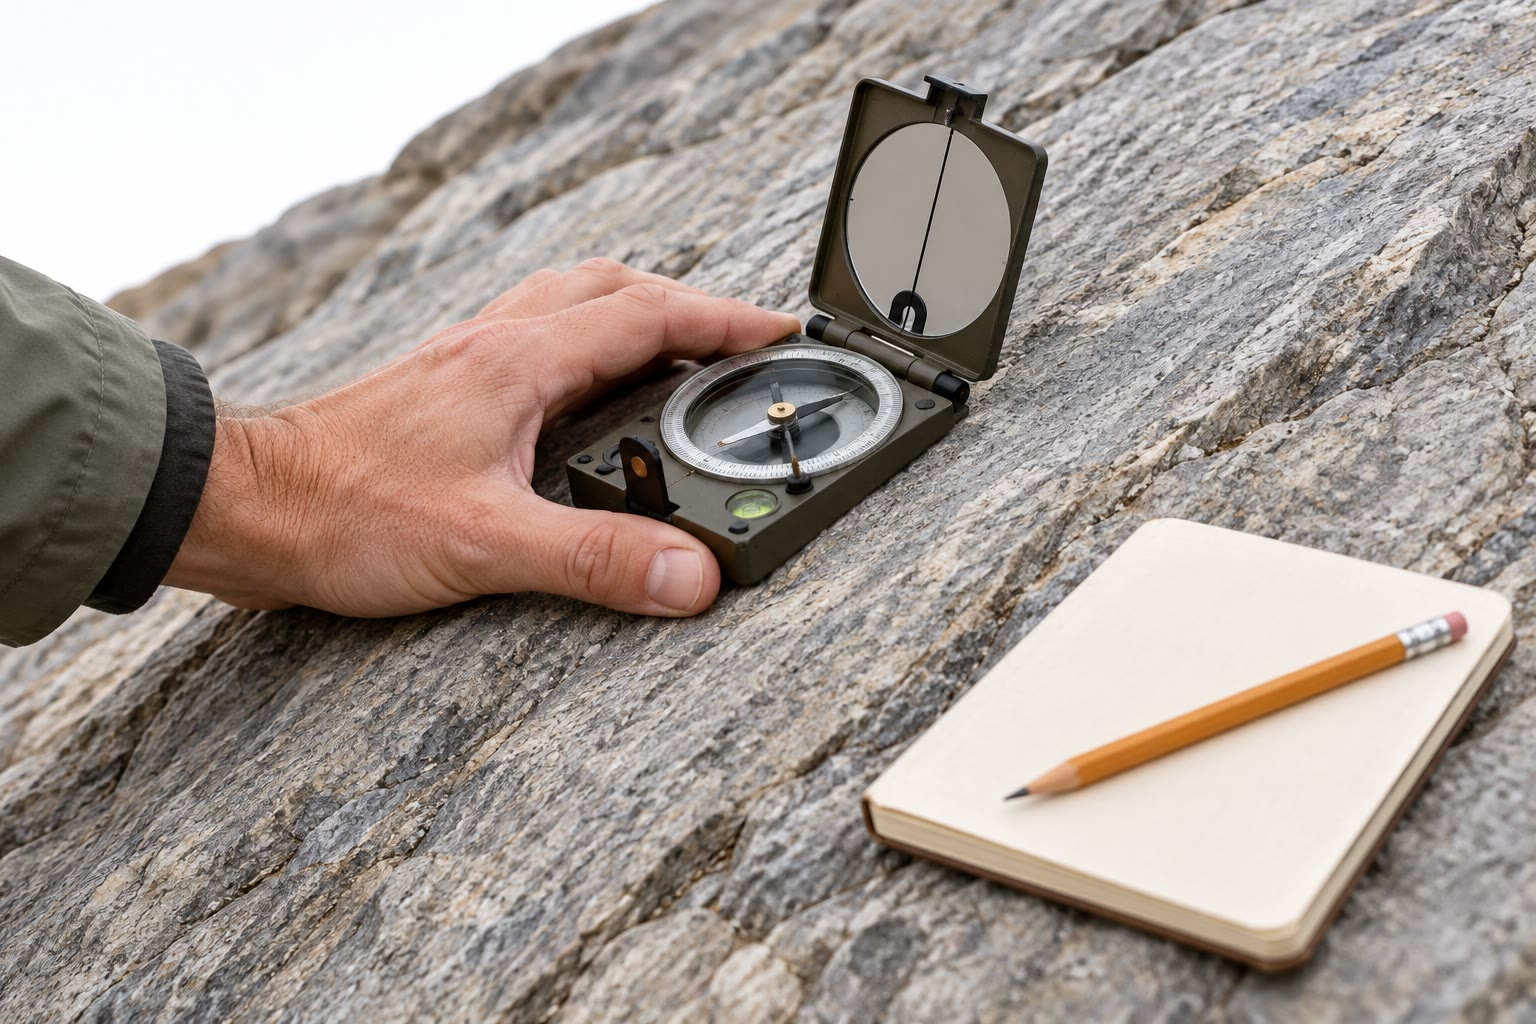
\includegraphics[width=\linewidth]{images/book5/ai/b3-compass-clinometer.jpg}

{\scriptsize Uma bússola-clinômetro apoiada contra uma superfície rochosa inclinada, com
um caderno de campo (ilustração gerada por IA).}
\end{minipage}
\end{inthefield}

\section{Exercícios}

\begin{exercise}[$\star$]\label{exo:b3:structural-analysis:1}
Determine o caimento e o trend do \omterm{def:b3:structural-analysis:stereo}{polo} do plano $040/30$ (direção de mergulho,
mergulho). Determine a atitude do plano cujo \omterm{def:b3:structural-analysis:stereo}{polo} tem trend \ang{315} e caimento
\ang{20}.
\end{exercise}

\begin{exercise}[$\star$]\label{exo:b3:structural-analysis:2}
Uma linha tem caimento \ang{30}. A que distância do centro ela se marca em uma \omterm{def:b3:structural-analysis:stereo}{rede de
ângulos iguais} e em uma rede de áreas iguais, ambas de raio \qty{10}{cm}?
\end{exercise}

\begin{exercise}[$\star$]\label{exo:b3:structural-analysis:3}
Os flancos de uma dobra têm as atitudes $090/30$ e $270/30$. Calcule o ângulo entre
seus \omterm{def:b3:structural-analysis:stereo}{polos} com o produto escalar das normais, o ângulo interflancos e a classe da
dobra.
\end{exercise}

\begin{exercise}[$\star$]\label{exo:b3:structural-analysis:4}
Uma falha $090/60$ tem estrias de \textit{rake} \ang{-45}. Com o vetor de direção
$\vec s = (0, 1, 0)$ e o vetor de mergulho máximo $\vec d$ do plano, o
deslizamento do bloco superior é $\vec u = \cos r\,\vec s - \sin r\,\vec d$. Calcule
$\vec d$, $\vec u$, e o trend e o caimento do deslizamento. Dê nome à falha.
\end{exercise}

\begin{exercise}[$\star\star$]\label{exo:b3:structural-analysis:5}
Os flancos de uma dobra têm as atitudes $060/40$ e $250/30$. Calcule o trend e o
caimento de seu eixo, e seu ângulo interflancos.
\end{exercise}

\begin{exercise}[$\star\star$]\label{exo:b3:structural-analysis:6}
Calcule a fração da área da rede que fica dentro do círculo das linhas com caimento
superior a \ang{60}, na rede de áreas iguais e na \omterm{def:b3:structural-analysis:stereo}{rede de ângulos iguais}, e a fração
das direções do hemisfério inferior com caimento superior a \ang{60}. Qual rede deve
ser usada para contar \omterm{def:b3:structural-analysis:stereo}{polos}?
\end{exercise}

\begin{exercise}[$\star\star$]\label{exo:b3:structural-analysis:7}
Três \omterm{def:b3:structural-analysis:stereo}{polos} estão no plano vertical leste--oeste, a \ang{-20}, $0$ e
\ang{20} da vertical: $\vec p = (\sin a, 0, -\cos a)$. Calcule o \omterm{def:b3:structural-analysis:orientation-tensor}{tensor de orientação},
seus autovalores e autovetores, e o \omterm{def:b3:structural-analysis:pi}{eixo beta}. Por que o menor autovalor é exatamente
zero?
\end{exercise}

\begin{exercise}[$\star\star$]\label{exo:b3:structural-analysis:8}
Marque no diagrama de Flinn o elipsoide $X : Y : Z = 3 : 1.5 : 1$, depois o elipsoide de
volume constante com $X = 1.8$ e $Y = 1.1$. Calcule $k$ para cada um e dê nome à
deformação.
\end{exercise}

\begin{exercise}[$\star\star$]\label{exo:b3:structural-analysis:9}
Em uma seção cortada paralela ao estiramento, ooides inicialmente redondos são
elipses de razão axial $2.25$, todas paralelas, e a área de cada uma permanece
inalterada. Calcule os estiramentos principais e a extensão ao longo do eixo longo.
Antes da deformação, os centros dos ooides nunca estavam mais próximos do que
\qty{0.4}{mm}: dê os semieixos do vazio do diagrama de Fry.
\end{exercise}

\begin{exercise}[$\star\star\star$]\label{exo:b3:structural-analysis:10}
A $\theta = \ang{60}$ do nadir, calcule o estiramento ao longo do raio,
$\mathrm dr/(R\,\mathrm d\theta)$, e ao redor do círculo, $r/(R\sin\theta)$,
para as duas projeções. Verifique o teorema sobre as projeções, e dê a razão entre
os eixos da oval em que a rede de áreas iguais transforma um círculo muito pequeno
ali.
\end{exercise}

\begin{exercise}[$\star\star\star$]\label{exo:b3:structural-analysis:11}
Em um regime transcorrente, $\sigma_1$ é horizontal para \ang{000},
$\sigma_3$ horizontal para \ang{090} e $\sigma_2$ vertical. Uma falha vertical tem
direção \ang{020}. Sem calcular $\vec\tau$, mostre que seu deslizamento é
horizontal para todo $\Phi$. Em seguida, calcule $-\vec\tau$ para $\Phi = 0.4$ com
a normal do plano $\vec n = (\cos\ang{20}, -\sin\ang{20}, 0)$ e dê o sentido do
deslizamento.
\end{exercise}

\begin{exercise}[$\star\star\star$]\label{exo:b3:structural-analysis:12}
Uma seção de \qty{20}{km} de comprimento corta um conjunto de dobras de descolamento.
Dois horizontes distantes \qty{1.0}{km} um do outro estão acima de seus níveis
originais pelas áreas \qty{6.0}{km^2} (inferior) e \qty{7.5}{km^2} (superior). Calcule o
encurtamento, a profundidade do descolamento abaixo do horizonte inferior, o
comprimento original da seção e sua variação relativa de comprimento.
\end{exercise}

\section{Problema: Dobras e falhas das Varden Hills}

\begin{problem}[{Problema de fim de semana --- o eixo de uma dobra, a paleotensão de um conjunto de falhas
e a restauração de uma seção, em uma região fictícia}]
\label{pb:b3:structural-analysis:1}
% values: calc/ch08.py; figdata/bachelor-3/stereonet.py (data invented from region.py)
Nas Varden Hills, a região fictícia da série, uma cobertura mesozoica repousa sobre um
embasamento de xisto e granito. A cobertura está dobrada em um anticlinal e um sinclinal verticais,
de flancos retos e depois cortada por uma falha normal. Um
geólogo mediu doze planos de acamamento nos dois flancos do anticlinal
(sentido de mergulho/mergulho, em graus):

\begin{center}
\small
\begin{tabular}{l|cccccc}
\hline
flanco leste & 075/13 & 084/11 & 089/13 & 079/14 & 086/12 & 072/11 \\
flanco oeste & 283/11 & 272/13 & 281/14 & 288/10 & 276/13 & 274/12 \\
\hline
\end{tabular}
\end{center}

As somas das normais unitárias voltadas para cima das seis medidas de cada flanco são
$\vec S_E = (1.2583, 0.2017, 5.8604)$ e $\vec S_W = (-1.2445, 0.1886,
5.8636)$ (leste, norte, para cima). Cinco falhas apresentam estrias (sentido de mergulho/mergulho,
\textit{rake} do deslizamento do bloco superior): $120/60/{-90}$ (a falha principal), $150/55/{-76}$,
$090/65/{-108}$, $200/70/{-78}$ e $060/50/{-105}$. A falha principal tem um
rejeito de \qty{200}{m}. Os eixos do anticlinal e do sinclinal estão separados por \qty{4}{km},
de modo que as dobras se repetem a cada \qty{8}{km} de leste a oeste.

\medskip\noindent\textbf{Parte I --- Polos e o eixo beta.}
\begin{enumerate}
  \item Dê o rumo e o caimento do \omterm{def:b3:structural-analysis:stereo}{polo} da medida $075/13$, e
        sua distância ao centro de uma rede de áreas iguais de raio
        \qty{10}{cm}.
  \item Calcule a normal unitária voltada para cima da medida $075/13$; verifique-a
        contra $\vec S_E$ em módulo.
  \item Calcule a atitude média de cada flanco a partir de $\vec S_E$ e $\vec S_W$,
        os comprimentos médios das resultantes e a dispersão quadrática média das
        medidas em torno de suas médias.
  \item Calcule $\vec S_E\times\vec S_W$, e o rumo e o caimento do
        \omterm{def:b3:structural-analysis:pi}{eixo beta}.
  \item Calcule o ângulo entre as duas normais médias, o ângulo interflancos,
        e a classe da dobra.
  \item O plano axial desta dobra simétrica contém o \omterm{def:b3:structural-analysis:pi}{eixo beta} e é
        perpendicular a $\vec m_E - \vec m_W$, a diferença entre as normais unitárias
        médias. Dê sua atitude; a dobra é vertical?
  \item Dê a atitude do cinturão $\pi$, e diga por que os \omterm{def:b3:structural-analysis:stereo}{polos} estão sobre
        ele.
\end{enumerate}

\medskip\noindent\textbf{Parte II --- O tensor de orientação.}
O \omterm{def:b3:structural-analysis:orientation-tensor}{tensor de orientação} dos doze \omterm{def:b3:structural-analysis:stereo}{polos} é
\[
  T = \begin{pmatrix} 0.04400 & 0.00035 & 0.00109\\ 0.00035 & 0.00144 & 0.03179\\
  0.00109 & 0.03179 & 0.95456 \end{pmatrix},
\]
com os autovalores $0.95562$, $0.04400$ e $0.00038$.
\begin{enumerate}[resume]
  \item Verifique que o traço de $T$ é 1. Com $\vec b = (0.0053, -0.9994,
        0.0333)$, o vetor unitário na direção de $\vec S_E\times\vec S_W$, calcule
        $\vec b^{\mathsf T}T\vec b$. O que o resultado diz sobre $\vec b$?
  \item Calcule o ângulo médio quadrático entre os \omterm{def:b3:structural-analysis:stereo}{polos} e o cinturão.
  \item Explique o valor de $\lambda_2$ a partir dos mergulhos dos flancos.
  \item A dobra é cilíndrica dentro da precisão das medidas?
  \item O caimento do \omterm{def:b3:structural-analysis:pi}{eixo beta} é fixado pela inclinação norte--sul do
        cinturão, para a qual cada \omterm{def:b3:structural-analysis:stereo}{polo} contribui com a dispersão encontrada na
        questão 9. Estime o erro padrão do caimento.
\end{enumerate}

\medskip\noindent\textbf{Parte III --- A paleotensão.}
\begin{enumerate}[resume]
  \item Que tipo de falha é a falha principal? Segundo Anderson, dê as
        direções de $\sigma_1$, $\sigma_2$ e $\sigma_3$.
  \item Mostre, com o teorema sobre a direção de deslizamento, que a falha principal
        desliza segundo a linha de máximo mergulho para todo valor de $\Phi$. O que isso
        revela sobre $\Phi$?
  \item Para a falha $150/55$, calcule $\vec n$ e suas componentes $n_1 =
        \vec n\cdot\vec e_1$ e $n_2 = \vec n\cdot\vec e_2$, com $\vec e_1$
        vertical e $\vec e_2$ horizontal apontando para \ang{030}.
  \item Seu deslizamento fornece $\vec w = \vec n\times\vec u = (0.771, 0.605, 0.198)$.
        Calcule $\Phi$.
  \item As outras três falhas menores dão $\Phi = 0.294$, $0.301$ e
        $0.306$. Dê a média e diga de onde vem a dispersão.
  \item O que $\Phi = 0.3$ diz sobre $\sigma_2$?
  \item Calcule os eixos P e T da falha principal (a \ang{45} do
        plano, no seu plano de mergulho), e compare-os com $\sigma_1$ e
        $\sigma_3$.
\end{enumerate}

\medskip\noindent\textbf{Parte IV --- Restauração de uma seção leste--oeste.}
\begin{enumerate}[resume]
  \item Calcule o mergulho aparente do flanco leste, $080.9/12.3$, em uma
        seção leste--oeste.
  \item Tomando os flancos a \ang{12} na seção, calcule o comprimento restaurado
        de um comprimento de onda da dobra, o encurtamento e a variação relativa
        de comprimento.
  \item Calcule a altura da crista do anticlinal acima dos sinclinais e a
        área excedente de um comprimento de onda, supondo que os sinclinais permaneceram
        no nível original.
  \item Calcule a profundidade do descolamento abaixo da camada dobrada. Podem as
        dobras estar descoladas na base da cobertura, a algumas centenas de metros
        abaixo?
  \item Calcule o afastamento horizontal e o deslizamento da falha principal em uma seção ao longo de
        \ang{120}.
  \item Na seção leste--oeste, calcule o mergulho aparente da falha e
        seu afastamento horizontal aparente. Qual seção deve ser restaurada?
  \item Em que ordem a falha e as dobras são restauradas, e onde são colocadas as
        \omterm{def:b3:structural-analysis:restoration}{linhas de fixação}?
  \item Qual é o caimento do eixo da dobra Varden, obtido a partir das doze
        medidas?
\end{enumerate}
\end{problem}
